\documentclass{article}
\usepackage[utf8]{inputenc}

\usepackage{float}
\usepackage{caption}

\RequirePackage{tabularx}



\usepackage[table]{xcolor} 
\definecolor{myblue}{HTML}{CCF4FF}
\definecolor{myorange}{HTML}{FCAD68}

\usepackage{tikz}
\tikzstyle{decision} = [diamond, draw, fill=myblue, 
text width=4.5em, text badly centered, node distance=2.5cm, inner sep=0pt]
\tikzstyle{block} = [rectangle, draw, 
fill=myblue, align=center, rounded corners, minimum width = 2cm, minimum height=1cm]
\tikzstyle{line} = [draw, -latex']

\usepackage{todonotes}
\setuptodonotes{inline}
\usepackage{quotes}

\newcommand{\quotes}[1]{``#1''}

\usepackage[table]{xcolor} 
\definecolor{myblue}{HTML}{CCF4FF}
\definecolor{myorange}{HTML}{FCAD68}

\usepackage{tikz}
\tikzstyle{decision} = [diamond, draw, fill=myblue, text width=4.5em, text badly centered, node distance=2.5cm, inner sep=0pt]
\tikzstyle{block} = [rectangle, draw, fill=myblue, align=center, rounded corners, minimum width = 2cm, minimum height=1cm]
\tikzstyle{line} = [draw, -latex']


\begin{document}


\pagestyle{empty}
\large

\section*{\centering\hspace{-1cm}3D printers - Handleiding}
Na deze handleiding weet je hoe je efficient 3D print aanvragen kan verwerken. Er wordt vanuit gegaan dat je al weet hoe de 3D printers werken, zoals materiaal vervangen, het bed schoonmaken, 3D bestanden slicen tot gcode en de meest voorkomende errors weet aan te pakken.\\

Na deze handleiding weet je ook hoe je gestructureerd en efficient 3D print aanvragen kan verwerken. Mail wordt vrijwel volledig geautomatiseerd beantwoorden en de continuiteit wordt behouden. Versta onder continuiteit, je kan meteen aan de slag en hoeft niet uit te zoeken wat je voorganger heeft gedaan voordat je aan de slag kan.\\


\section*{Termologie}
\noindent\textbf{Een print job}: Een folder met daarin alle bestanden gerelateerd aan het .stl file, deze gerelateerde bestanden kunnen zijn: een mail gesprek, gcode, een van de~.exe functies (\textit{afgekeurd.exe}, \textit{gesliced.exe}, \textit{printer\_aangezet.exe} of \textit{printer\_klaar.exe}), of overige bestanden. Een print job wordt aangemaakt door de \textit{inbox.exe} functie vanuit de mail inbox, of via de \textit{selecteer\_bestand.exe} functie.\\

\todo{welke andere }


\section*{Globaal Overzicht}
Een 3D print aanvraag wordt omgezet tot een \quotes{print job}, dit is een folder met daarin alle bestanden die bij een 3D print aanvraag horen. 


\todo{maak een actie bolletjesc}

Door batch files aan te roepen (batch file met extensie .bat roept een python script aan) kan je 


Er zijn vijf folders, deze \todo{laat SA naar folders kijken}




\begin{center}
\scalebox{0.7}{
  \hspace{0.5cm}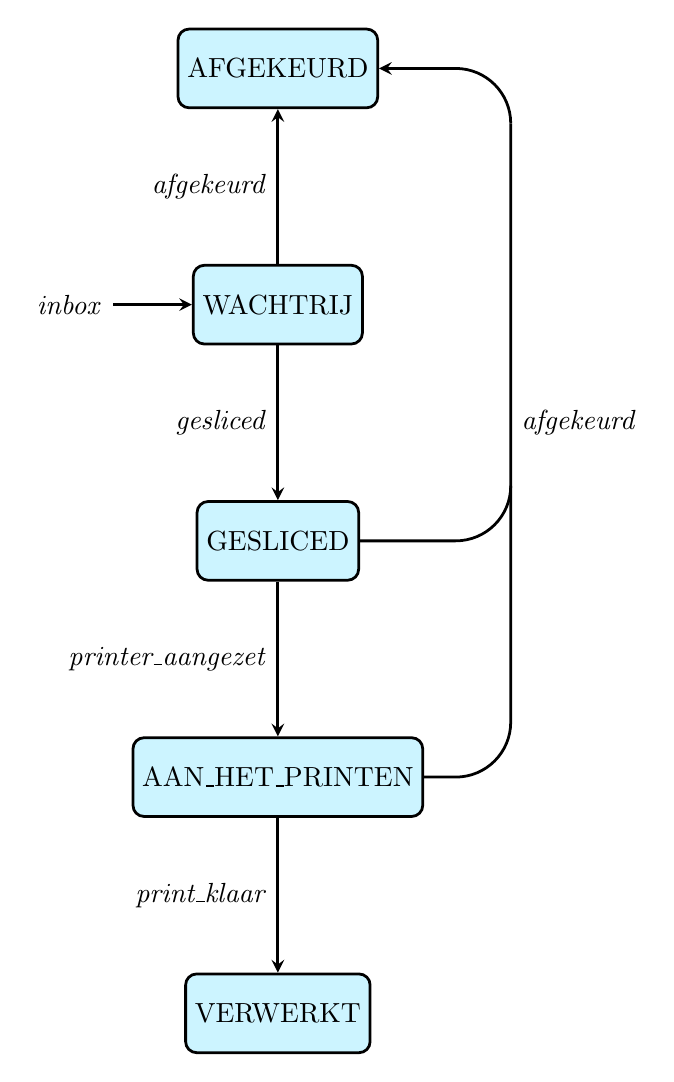
\begin{tikzpicture}[node distance = 3.0cm, line width=1pt]
    % Nodes
    \node [block] (wachtrij) {WACHTRIJ};
    \node [block, above of=wachtrij]  (afgekeurd) {AFGEKEURD};
    \node [block, below of=wachtrij]  (gesliced) {GESLICED};
    \node [block, below of=gesliced]  (aan_het_printen) {AAN\_HET\_PRINTEN};
    \node [block, below of=aan_het_printen] (verwerkt) {VERWERKT};

    % define lengths
    \pgfmathsetlengthmacro{\alpha}{0.7cm} % curve radius
    \pgfmathsetlengthmacro{\negalpha}{-\alpha}
    \pgfmathsetlengthmacro{\beta}{0.4cm} % straight bit before the curve

    % arrows
    \draw[>=stealth, ->, line width=1.0pt] ([xshift=-1.0cm]wachtrij.west) to node[xshift=-0.5cm,left]{\textit{inbox}} (wachtrij.west);
    \draw[>=stealth, ->, line width=1.0pt] (wachtrij.north) to node[left] {\textit{afgekeurd}} (afgekeurd.south);
    \draw[>=stealth, ->, line width=1.0pt] (wachtrij.south) to node[left] {\textit{gesliced}} (gesliced.north);
    \draw[>=stealth, -, line width=1.0pt] (aan_het_printen.east) -- ++(\beta,0)  to[out=0, in=-90] ++(\alpha, \alpha) -- node[right]{\textit{afgekeurd}} ([xshift=\alpha+\beta,yshift=\negalpha]afgekeurd.east -| aan_het_printen.east);
    \draw[>=stealth, <-, line width=1.0pt] (afgekeurd.east) -- ([xshift=\beta] afgekeurd -| aan_het_printen.east)  to[out=0, in=90] ++(\alpha,\negalpha);
    \draw[>=stealth, -, line width=1.0pt] (gesliced.east) -- ([xshift=\beta] gesliced -| aan_het_printen.east) to[out=0, in=-90] ++(\alpha,\alpha);
    \draw[>=stealth, ->, line width=1.0pt] (gesliced.south) to node[left] {\textit{printer\_aangezet}} (aan_het_printen.north);
    \draw[>=stealth, ->, line width=1.0pt] (aan_het_printen.south) to node[left] {\textit{print\_klaar}} (verwerkt.north);

  \end{tikzpicture}

}
\end{center}

\section*{Functie Beschrijving:}

\todo{Update deze functie beschrijvingen}


\section*{Let Hier Op!}
niet wegklikken van cmd




Je bent klaar! Optioneel kan je het overzicht van de batch files doorlezen.\\

\begin{table}[H]
\hspace{-2cm}
    \rowcolors{2}{gray!25}{white}
    \begin{tabular}%
    {>{\raggedright\arraybackslash}p{0.25\textwidth}%
    |>{\raggedright\arraybackslash}p{1.05\textwidth}}
    \rowcolor{myblue}
    Functie & beschrijving\\\hline

  \textit{inbox.exe}& Vraag of alle \textit{x} binnengekomen mails of een enkele ($x=1$) mail behandeld moet worden. Bij een enkele mail selecteer welke via interactief keuzemenu in de terminal. Maak voor iedere mail die .stl bestanden bevat een folder WACHTRIJ/\textit{naam}/ aan waarbij \textit{naam} de naam is van de persoon die de mail heeft gestuurd. Download de .stl attachments en de binnen gekomen mail naar de respectivelijke \textit{naam} folder. Maak voor ieder van de \textit{x} folders de \textit{gesliced.exe} en \textit{afkeur.exe} functies en plaats deze in de respectivelijke WACHTRIJ/\textit{naam}/ folder.\\

\textit{selecteer\_bestand.exe}& Deze functie is wachtwoord beveiligd, voer eerst het wachtwoord in. Open verkenner om een locale folder of 3D print bestand te selecteren. Vraag interactief om een \textit{naam} in te voeren, maak een folder WACHTRIJ/\textit{naam}/ en verplaats de inhoud van de geselecteerde folder of 3D print bestand naar folder \textit{naam}. Maak de \textit{gesliced.exe} en \textit{afkeur.exe} functies en plaats deze in de WACHTRIJ/\textit{naam}/ folder.\\

\textit{afgekeurd.exe}& 
Maak de folder AFGEKEURD/\textit{MM}-\textit{DD}\_\textit{naam}/ hierbij is \textit{MM-DD} vandaag. Verplaats de inhoud van de folder waarin \textit{afgekeurd.exe} zich bevind van de WACHTRIJ, GESLICED of AAN\_HET\_PRINTEN folder naar de AFGEKEURD/\textit{MM}-\textit{DD}\_\textit{naam}/ folder en verwijder de lege folder. Als er een mail thread in de folder zit, popup een mail reactie voor met de `afkeur' handtekening voor de SA om aan te passen en te versturen.\\

\textit{gesliced.exe}& Maak de folder GESLICED/\textit{hh}h\_\textit{mm}m\_\textit{naam}/ hierbij is \textit{hh} het aantal uren van de print en \textit{mm} het aantal minuten van de print. Verplaats de inhoud van WACHTRIJ/\textit{naam}/ (waarin \textit{gesliced.exe} zich bevind) naar de GESLICED/\textit{hh}h\_\textit{mm}m\_\textit{naam}/ folder, verwijder de lege folder. Maak een \textit{printer\_aangezet.exe} functie en plaats deze in de GESLICED/\textit{hh}h\_\textit{mm}m\_\textit{naam}/ folder.\\

\textit{printer\_aangezet.exe}& 
Maak de folder AAN\_HET\_PRINTEN/\textit{MM}-\textit{DD}\_\textit{hh}h\_\textit{mm}m\_\textit{naam}/ waarbij \textit{MM-DD} vandaag is. Verplaats de inhoud van GESLICED/\textit{hh}h\_\textit{mm}m\_\textit{naam} (waarin \textit{printer\_aangezet.exe} zich bevind) naar de AAN\_HET\_PRINTEN/\textit{MM}-\textit{DD}\_\textit{hh}h\_\textit{mm}m\_\textit{naam} folder en verwijder lege de GESLICED/\textit{hh}h\_\textit{mm}m\_\textit{naam} folder. Maak de \textit{print\_klaar.exe} functie en plaats deze in de AAN\_HET\_PRINTEN/\textit{MM}-\textit{DD}\_\textit{hh}h\_\textit{mm}m\_\textit{naam}/ folder.\\

\textit{print\_klaar.exe}& Maak de folder VERWERKT/\textit{MM}-\textit{DD}\_\textit{hh}h\_\textit{mm}m\_\textit{naam}/ en verplaats de inhoud van AAN\_HET\_PRINTEN/\textit{MM}-\textit{DD}\_\textit{hh}h\_\textit{mm}m\_\textit{naam} (waarin \textit{print\_klaar.exe} zich bevind) naar de VERWERKT/\textit{MM}-\textit{DD}\_\textit{hh}h\_\textit{mm}m\_\textit{naam} en verwijder lege de folder. Als er een mail thread in de folder zit, popup een mail reactie met de `print klaar' handtekening voor een SA om aan te passen en te versturen.\\

    \end{tabular}
    % \caption*{}%
\end{table}



\end{document}


